\documentclass[a4paper,USenglish]{socg-lipics-v2018}
\usepackage{amsthm}
\usepackage{amsmath}
\usepackage{mathbbol}
\usepackage{amsfonts}
\usepackage{amssymb}
\usepackage{graphicx}
\usepackage{algorithm}
\usepackage{url}
%\usepackage{floatflt}
%\usepackage{mathptmx}
\usepackage{epsfig}
\usepackage{wrapfig}
\usepackage{color}

\usepackage{algorithm}
\usepackage[noend]{algpseudocode}
\usepackage{comment}
\usepackage{braket}

% \usepackage{ccaption}

\newcommand{\N}{\mathbb{N}}
\newcommand{\Q}{\mathbb{Q}}
\newcommand{\R}{\mathbb{R}}
\newcommand{\Z}{\mathbb{Z}}
\renewcommand{\S}{\mathbb{S}}
\newcommand{\dappr}{\tilde{d}}
%\newcommand{\Wlog}{W.l.o.g.\ }
%\newcommand{\wlog}{w.l.o.g.\ }
\newcommand{\eps}{\varepsilon}
\newcommand{\orient}{O}
\newcommand{\cpro}{\Pi}
\newcommand{\fib}{\mathrm{Fib}}

\newcommand{\metricspace}{\mathcal{M}}
\newcommand{\approxmetric}{\gamma}
\newcommand{\parent}{\mathrm{par}}
\newcommand{\point}{p}
\newcommand{\level}{\ell}
\newcommand{\diam}{\mathrm{diam}}
\newcommand{\pointset}{P}
\newcommand{\distspace}{\mathcal{M}}
\newcommand{\dist}{\delta}
\newcommand{\adist}{\gamma}
\newcommand{\complexity}{C_{\dist}}
\newcommand{\doublingdimension}{\Delta}

%\newcommand{\remark}[1]{\textbf{[#1]}}

%\newtheorem{theorem}{Theorem}
%\newdef{definition}{Definition}
%\newtheorem{lemma}[theorem]{Lemma}
%\newtheorem{corollary}[theorem]{Corollary}

\newcommand{\myparagraph}[1]{\textbf{#1.}}

%\newtheorem{theorem}{Theorem}
%\newtheorem{lemma}[theorem]{Lemma}
%\newtheorem{proposition}[theorem]{Proposition}
%\newtheorem{corollary}[theorem]{Corollary}
%\newtheorem{definition}[theorem]{Definition}
%\newtheorem{remark}[theorem]{Remark}
%\newtheorem{note}[theorem]{Note}

%\numberwithin{equation}{section}
%\numberwithin{figure}{section}

\def\marrow{\marginpar[\hfill$\longrightarrow$]{$\longleftarrow$}}
\def\michael#1{\textcolor{red}{\textsc{Michael says: }{\marrow\sf #1}}}

\title{Metric Spaces with Expensive Distances}
\author{Michael Kerber}{TU Graz}{kerber@tugraz.at}{}{}
\author{Arnur Nigmetov}{TU Graz}{nigmetov@tugraz.at}{}{}
\authorrunning{M. Kerber and A. Nigmetov}

\keywords{metric spaces, doubling dimension, spanners, approximate nearest neighbor}
\subjclass{dummy}
% \category{dummy}

\Copyright{Michael Kerber and Arnur Nigmetov}

\begin{document}
\maketitle

\begin{abstract}
In algorithms for finite metric spaces, it is common
to assume that the distance between two points
can be computed in constant time, and complexity
bounds are expressed only in terms of the number
of points of the metric space.
We introduce a different model where we assume
that the computation of a single distance is
an expensive operation and consequently, the goal is
to minimize the number of such distance queries.
This model is motivated by metric spaces
that appear in the context of topological data analysis.

We consider two standard operations on metric spaces,
namely the construction of an $\epsilon$-spanner
and the computation of an approximate nearest
neighbor for a given query point.
In both cases, we partially explore the metric space
through distance queries and infer lower and upper bounds
for yet unexplored distances through triangle inequality.
For spanners, we evaluate several exploration strategies
through extensive experimental evaluation.
For approximate nearest neighbors, we prove that our
strategy returns an approximate nearest neighbor
after a logarithmic number of distance queries.
\end{abstract}

\section{Introduction}

Given a set $\pointset:=\{p_1,\ldots,p_n\}$ of $n$ points
in a metric space $(\metricspace,\dist)$, 
consider the following standard operations:

\begin{description}
\item[Approximate Nearest Neighbor] Given $\eps>0$ and a point $q\in\metricspace$,
find $p_i\in\pointset$ such that, for all $j=1,\ldots,n$,
\[\dist(q,p_i)\leq(1+\eps)\dist(q,p_j)\]

\item[Spanner] Given $\eps>0$, compute a weighted graph $G$ with vertices in $\pointset$
such that for any $u,v\in\pointset$, the shortest path distance between $u$ and $v$
is at most $(1+\eps)\dist(u,v)$.
\end{description}


The performance of algorithms for these problems depends on the number of points,
the dimension of the metric space, and the cost $\complexity$ of computing a distance in the metric space.
It is a common assumption to assume $\complexity$ to be a constant; 
There are good reasons for that: the most common case of a metric space
is $\metricspace=\R^d$ with $d$ some constant, in which case $\complexity$ can be evaluated in $O(d)=O(1)$ time.
Even if $d$ is considered non-constant,
it can always be assumed that $d\leq n$, hence $\complexity$ is at most $O(n)$.
Another typical assumption is that all pairwise distances are part of the input
in which case $\complexity$ is $O(1)$.

However, we argue that in some situations, distance computations
in $\metricspace$ can be costly and $\complexity$ might be incomparable
with $n$. Our motivation comes from topological summaries
such as persistence diagrams or Reeb graphs, which are of interest
in the field of topological data analysis. A persistence diagram
is a point set in $\R^2$, and the distance between two diagrams
is determined by a min-cost matching between the point sets.
If the diagrams have $N$ points, computing this matching requires
polynomial time in $N$, and $N$ might well be larger than $n$, the number
of diagrams considered. For the case of Reeb graphs, the situation is even
worse: while several metrics on Reeb graphs have been proposed,
not even an constant-factor approximation algorithm is known that runs
in polynomial time in the size of the graphs.
\michael{This paragraph needs references. As you know the literature better than me,
I leave that part to you.}

In such situations with expensive distance computations, 
it makes sense to study a different cost model, where only the number of distance computations
is taken into account. For instance, that means that quadratic time operations in terms of $n$
are not counted towards the time complexity, as long as these operations do not query any distance
in $\metricspace$. We also ignore the space complexity in our model.

We will restrict to the case of \emph{doubling spaces}, that is, the doubling dimension
of $\metricspace$ is bounded by a constant. 
In that situation, standard constructions from computational geometry provide partial answers:
Using net-trees~\cite{hm-fast}, we can construct a $\eps$-well-separated pair decomposition (WSPD)~\cite{CK-decomposition} using $O(n\log n)$ distance queries; a WSPD in turn yields
an $\eps$-spanner immediately. Net-trees can also be used to compute approximate nearest neighbors
performing $O(\log n)$ distance computations per query point.
However, for our relaxed cost model, we pose the question whether simpler constructions achieve
comparable, or even fewer distance computations.

We also propose a slight variant of our model: we assume that we also have access to an (efficient)
$2$-approximation algorithm for the distance queries. Queries to this approximation algorithm
are not counted in the model, hence we can assume that for each pair of points $(u,v)$, we
know a number $a_{u,v}$ with $\dist(u,v)\leq a_{u,v}\leq 2\dist(u,v)$. This induces an approximate ordering
of all distances in the metric space, and it is plausible to assume that such an ordering will simplify
algorithmic tasks on metric spaces, at least in practice.

\myparagraph{Contributions}
%
We propose simple algorithms for spanner construction and approximate nearest neighbor search
and evaluate them theoretically and experimentally in the defined cost model.

Our algorithms are based on the following simple idea: since distance computations are expensive
and should be avoided, we try to obtain maximal information out of the distances that have been computed
so far. 
This information consists of lower and upper bounds for unknown distances, obtained from known distances
by triangle inequality (see Figure~\ref{fig:1st_example}). We remark that updating these bounds involves $\Omega(n^2)$ arithmetic
operations whenever a new distance has been computed, turing the method useless in the standard computational model.

\begin{figure}[h]
\centering
\includegraphics[width=6cm]{intro_example.eps}
\caption{The compute distances are shown as edges in a graph. Note that the exact distance
of $p_1$ and $p_2$ is unknown. The shortest path from $p_1$ to $p_2$ has length $9$, which clearly
constitutes an upper bound on the distance by triangle inequality.
However, we can also infer that $\dist(p_1,p_2)\geq 3$:
otherwise, the path from $p_3$ to $p_4$ via $p_1$ and $p_2$
would be shorter than the edge $(p_3,p_4)$, again contradicting
triangle inequality.}
\label{fig:1st_example}
\end{figure}

We propose several heuristics of how to explore the metric space to obtain accurate lower and upper bounds
with a small number of distance computation. Once the ratio of upper and lower bound is at most $(1+\eps)$
for each point pair, the set of all computed distances forms the spanner.
The experimentally most succesful exploration strategy that we found is to
repeatedly query the distance of a pair with the worst ratio of upper and lower bound.
We call the obtained spanner the \emph{blind greedy spanner}, as opposed to the well-known
\emph{greedy spanner} that precomputes all pairwise distances and only maintains upper bounds.\michael{Cite}
Remarkably, we were not able to improve the quality when knowing initial $2$-approximations of all point pairs.
\michael{Acutally, is that true? We could run BlindGreedy on the 2-approximations instead of on $[0,\infty]$,
that might save something}
We also compare with a spanner construction based on WSPDs. Our simple algorithms tend to give much smaller
spanners on the tested example. Nevertheless, we leave the question open whether our construction
yields a spanner of asymptotically linear size.

For approximate nearest neighbor, we devise a simple randomized incremental algorithm and show that
the number of distance queries to find an approximate nearest neighbor is $O(\log n)$ in expectation.
Our proof is based on the well-known observation that the nearest neighbor changes $O(\log n)$ times
in expectation when traversing the sequence of points, combined with a packing argument certifying that
only a constant number of distances needs to be computed in-between two minima.
We also experimentally evaluate our approach and observe that the approach follows 
roughly the theoretical prediction.



\section{Notation and Preliminary Notions}
Let $(X, \dist)$ be a finite metric space with $n$. Let $G$ be a graph with set of vertices $X$,
its edges have natural weighting $w(x,y) = \dist(x, y)$ which induces the graph metric $\dist_G$ on $X$.
Graph $X$ is called a $1 + \eps$-spanner of $P$, if $\dist_G$ is a good approximation of $\dist$:
$\dist(x,y) \leq \dist_G(x, y) \leq (1+\eps) \dist(x, y)$. Obviously, $G$ must have $\Omega(n)$ edges,
and we consider $G$ optimal, if it has $O(n)$ edges (for each edge of $G$ we must compute the corresponding
distance, if we want to use the spanner instead of the original metric, which dictates this
choice of optimality measure). 



A metric space is called \textit{doubling} with \textit{doubling constant} $k$,
if every ball of radius $r$ can be covered by at most $k$ balls of radius $r/2$,
and $k$ is the smallest number having that property.
\textit{Doubling dimension} of a doubling space is defined as $\log k$
(since we usually ignore multiplicative constants, the base of the logarithm is not really important; however,
we always use $\log$ to denote the logarithm with base 2).
It is easy to see that a subspace of a space with doubling dimension $d$ 
is always doubling and has the doubling dimension $O(d)$ (but not necessarily $d$).


In this paper we consider some fixed metric space $(X, \dist)$, and, to get interesting
results we must assume doubling property.

We shall need the following lemma, which is just a reformulation of the well-known
packing lemma for doubling spaces (see \cite{smid_2009}, Sect. 2.2).

\begin{lemma}
\label{lem:packing_lemma}
 Let $(X,\dist)$ be a metric space of doubling dimension $d$, and let $P$ be a subset of a ball 
 $B(x,R)$ in $X$ such that the distance between any two distinct points of $P$ is at least $r$.
 Then $P$ is finite and its cardinality is bounded by some $C$ that depends only on $d$
 and the ratio $r/R$.
% Then $P$ is finite and cardinality of $P$ satisfies the inequality $|P| < 2^{md}$, where $m = 1 + \lceil \log (R/r) \rceil $. 

% Let $(X,\dist)$ be a metric space of doubling dimension $d$, and let $P$ be a subset of a ball $B(x,R)$ in $X$ such that the distance between any two distinct points of $P$ is at least $r$.
% Then $P$ is finite and cardinality of $P$ satisfies the inequality $|P| < 2^{md}$, where $m = 1 + \lceil \log (R/r) \rceil $. 
\end{lemma}
\begin{proof}
We can cover $B(x,R)$ with $2^d$ ball of radius $R/2$, each of these balls we can cover with $2^d$
balls of radius $R/4$, etc. Repeating this process $m := \lceil \log \frac{R}{r/2} \rceil$ times, 
we cover
$B(x, R)$ with $2^{md}$ balls of radius at most $r/2$. Since a ball of radius $r/2$ can
contain at most one point from $P$, the claim follows.
\end{proof}
If the doubling dimension of $(X, \dist)$ is larger than $d$, then
there exists a ball of radius $R$ such that there are at least $2^d$ points with pairwise distance at least $R$. On the other hand,
the maximal distance between any two of these points is at most $2R$, and we have a lot of points with approximately the same distance
between them. If we want a high-quality spanner on these points, then we can expect that its size will be quadratic, not linear;
so the space of high doubling dimension cannot have optimal spanners. Thus the question of approximating
the non-doubling metric without computing many distances cannot be solved positively, and we should
restrict our attention to the case of doubling spaces.

\section{Metric Approximation}

It is known that optimal spanner can be constructed by the following greedy algorithm: 
start with an empty graph on vertices $p_i$,
sort all edges $\{p_i, p_j\}$ by the length $\dist(p_i, p_j)$ in ascending order and keep adding them to the graph
until it becomes a $1+\eps$-spanner. 


 In our setting this is the most expensive approach, because it requires
 computing all pairwise distances first. We propose an alternative approach (or rather a family of algorithms), which we call
 \textit{blind} spanner, meaning that the algorithm that builds a spanner does not have access to $\dist(p_i, p_j)$
 before it decides to add the edge $(p_i, p_j)$.
 The algorithm also maintains lower and upper bounds
 for all pairwise distances, which are updated after a new edge is added.
 These bounds are used in the stopping criterion, namely, if $a_{i, j}$ and $b_{i,j}$ denote lower and upper bounds
 for the distance between $p_i$ and $p_j$, respectively, 
 then the algorithm stops, if $b_{i,j} / a_{i, j} \leq 1 + \eps$
 for all $i \neq j$.

\begin{algorithmic}
\label{alg:blind_spanner}
\Function{BlindSpanner}{$P, \eps$}
    \State {$E \gets \emptyset$}
    \State {$a_{i,j} \gets 0$ for all $1 \leq i,j \leq n$}
    \State {$b_{i,j} \gets \infty$ for all $1 \leq i,j \leq n, i \neq j$}
    \While {$\exists i \neq j : b_{i,j} / a_{i,j} > 1 + \eps$}
    \State {$(i,j) \gets $} \Call{GetEdgeToAdd}{}
    \State {$v \gets \dist(p_i, pj)$}
    \State {Add weighted edge $(p_i, p_j, v)$ to $E$}
    \State \Call{UpdateBounds}{$i, j, v$}
    \EndWhile
\EndFunction
\end{algorithmic}


In this pseudocode we adopt the convention that a positive number divided by 0 is $\infty$
and $\infty$ is larger than any real number,
thus making the predicate in the while loop well-defined.  The procedure \textsc{UpdateBounds} is described in the next subsection,
now we only mention that it updates all upper and lower bounds based on triangle inequality involving the edge $(p_i, p_j)$,
and the update is monotonic: no upper bound can increase, no lower bound can decrease, and, after the distance
between $p_i$ and $p_j$ is calculated, both $a_{i,j}$ and  $b_{i,j}$ are set to be $\dist(p_i, p_j)$.
The most important part of this algorithm is the way of choosing the next edge to be added, and
there are several possibilities, which give very different results.



The first possibility will be called \textsc{BlindGreedy}, where we choose a pair $(p_i, p_j)$ that maximizes
the ratio $b_{i,j} / a_{i,j}$. If the number of maximizing pairs is more than 1, we choose one of them at random.
Note that our conventions imply that in \textsc{BlindGreedy} the edges that have $a_{i,j} = 0$ or $b_{i,j} = \infty$
have the highest priority, so the algorithm first ensures that the graph is connected and there are positive
lower bounds for every edge before it will start adding any other edges.



The second possibility will be referred to as \textsc{BlindRandom}, where among all edges $(p_i, p_j)$
for which $b_{i,j} / a_{i,j} > 1 + \eps$ we choose one uniformly at random. We may vary this approach
by insisting that we must first create a connected graph, or that we must first have some positive lower bound
for all edges, and only after these requirements are satisfied, we consider other pairs.



The last option that we consider is based on an additional assumption: while
computing $\dist(\cdot, \cdot)$ exactly is costly, we have access to a
cheap approximation algorithm
that gives a $2$-approximation of $\dist$ much faster 
(the output of this approximation algorithm is guaranteed to
lie in $[\dist(p,q), 2 \dist(p,q)]$). In order to simplify notation, we now assume
that all pairwise distances between our points belong to $[1, 2^t]$ for some $t$.
We introduce \textit{buckets} of the form $[2^k, 2^{k+2}]$ for $k = 0 \dots t$;
these intervals are not disjoint, but by calling the approximation algorithm we can assign
each pair $(p_i, p_j)$ to one of the buckets.
Indeed, let $v$ be the output of the approximation algorithm for $\dist(p,q)$,
then we know that the true distance is in $[v/2, v]$. We want to put the pair $(p,q)$ into the bucket
that fully contains this interval, thus we need to find $k$ such that
$2^k \leq v /2$ and $v \leq 2^{k+2}$. These inequalities give $ 2^{k+1} \leq v \leq 2^{k+2}$,
and we take $k = \lfloor \log v \rfloor - 1$.
Afer we found a bucket for each pair $(p_i, p_j)$, 
we have some sort of a weak ordering: we cannot say anything
about two edges that are assigned to the same bucket or to overlapping buckets, but if the buckets
are disjoint, we know which edge is longer. Now we can either imitate the greedy spanner (non-blind) algorithm,
traversing buckets in the order of their left endpoint, and adding edges from them; or we could alternate: in even iterations
we traverse the buckets from left to right, adding edges from each bucket one by one, and in odd iterations
we traverse the buckets from right to left. This alternative makes sense, because we need to have good lower bounds in
order to build a blind spanner, and good lower bounds can be obtained from the triangle inequality, if one of the edges 
in a path connecting $p_i$ and $p_j$ in $G$ is longer than the sum of the lengths of all other edges.
We refer to the former option as \textsc{BlindQuasiSortedGreedy} and to the latter one as \textsc{BlindQuasiSortedShaker}.


 \subsection{Maintaining Lower and Upper Bounds}

 In this subsection we explain the update procedure that we use. Suppose that
 $a_{k,l}$ and $b_{k,l}$ are valid lower and upper bounds, so that
\[
     \forall 1 \leq k < l \leq n \quad a_{k,l} \leq \dist(p_k, p_l) \leq b_{k,l}.
\]
Assume that $\dist(p_i,p_j)=v\in\R$ has been computed.
First, we reset $a_{i,j}$ and $b_{j,i}$ to $v$. 
To update the upper bound of some entry $b_{k,\ell}$,
we observe that the shortest path from $p_k$ to $p_\ell$ might now
go through the new edge. Hence, we update
\[
    b_{k,\ell}\gets \min_{i,j}\{b_{k,\ell},b_{k,i}+v+b_{j,\ell},b_{k,j}+v+b_{i,\ell}\}
\]
Repeating this for all $k,\ell$ yields the updated upper bounds in $O(n^2)$
time per entry.

For the lower bound, we observe that for any $1\leq k,\ell\leq n$,
\[
    v-b_{k,i}-b_{\ell,j}
\]
is a lower bound for $\dist(p_k,p_\ell)$. Indeed, this follows from
the triangle inequality
%
\[\dist(p_i,p_j)\leq \dist(p_i,p_k)+\dist(p_k,p_\ell)+\dist(p_\ell,p_j)\]
by rearranging terms and plugging in the upper bounds for $\dist(p_i,p_k)$
and $\dist(p_k,p_\ell)$. An analogue bound holds with $i$ and $j$ swapped. Hence, we update
%
\[a_{k,\ell}\gets \max\{a_{k,\ell},v-b_{k,i}-b_{\ell,j},v-b_{k,j}-b_{\ell,i}\}\]
%
for all $k,\ell$.

% Note that after we added the edge $(p_i, p_j)$, the ratio of the upper and lower bound
% for this pair becomes 1, so a blind spanner algorithm always terminates (of course,
% we assume that the procedure \textsc{GetEdgeToAdd} picks an edge only once).


\subsection{Experimental Results}
At the moment we cannot provide any theoretical guarantees for the heuristics that we propose to compute blind spanners,
and it can happen that it will yield the complete graph as a spanner.
We run experiments on the points sampled from the low-dimensional Euclidean space to investigate
experimentally the performance of these heuristics. Clearly, this has no practical meaning for $\R^d$, but
this space is well-suited for controlled experiments.

\begin{figure}[ht]
    \label{fig:spanner-sparseness}
    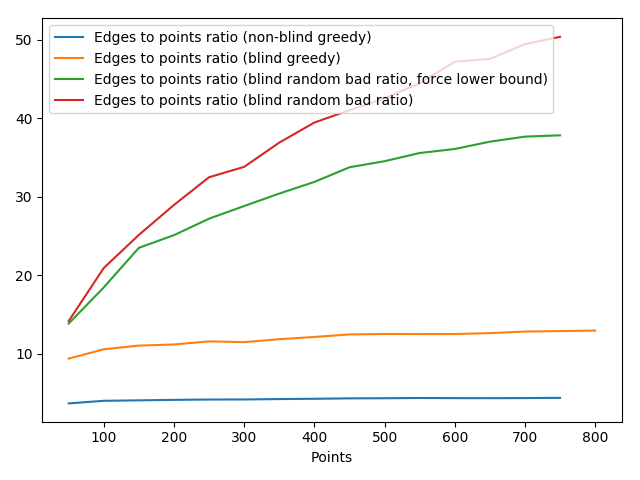
\includegraphics[width=0.7\textwidth]{pics/edges_to_points_ratio_dim_2_normal_points.png}
    \caption{Number of edges in blind spanners generated by different variants of the blind
    algorithm. Greedy non-blind algorithm is included for comparison. The plot is for normally distributed points
    in dimension 2, $\eps = 0.1$.}
\end{figure}

\begin{figure}[ht]
    \label{fig:blind-greedy-only}
    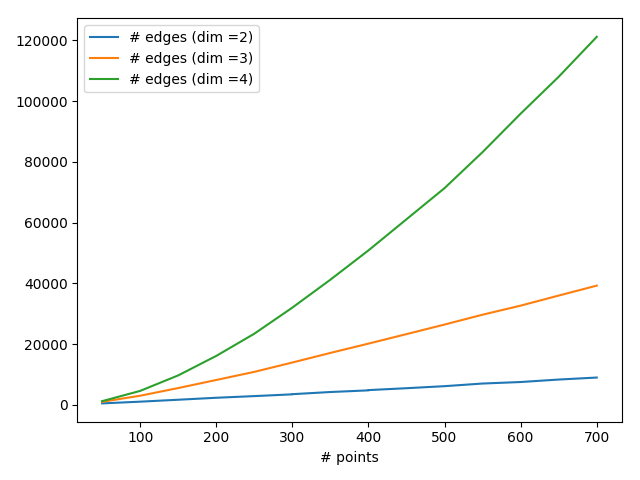
\includegraphics[width=0.7\textwidth]{pics/blind-greedy-dims.png}
    \caption{}
\end{figure}

\begin{figure}[ht]
    \label{fig:blind-rbr-variants}
    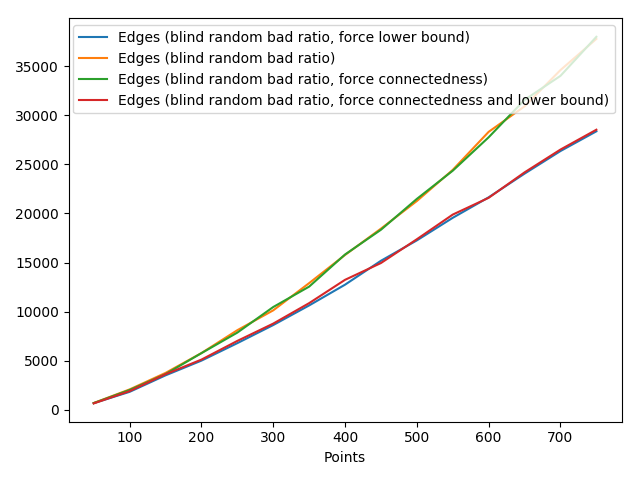
\includegraphics[width=0.7\textwidth]{pics/random-bad-ratio-comparison.png}
    \caption{Comparison of the four variants of \textsc{BlindRandomBadRatio} algorithm.}
\end{figure}

We tested the algorithm for $\eps \in \Set{0.01, 0.1, 0.2, 0.5}$ on the following sets of points in dimensions $d = 2,3,4,5$:
\begin{enumerate}
    \item In the \textbf{uniform} test set points are sampled uniformly at
        random from the unit cube in $\mathbb{R}^d$.
    \item In the \textbf{normal} test set points are sampled from the standard
        normal distribution in $\mathbb{R}^d$.
    \item In the \textbf{clustered} test set we first sample cluster centers uniformly 
        at random from $[0,10000]^d$, and then we add normally distributed noise around
        each of the centers. The number of clusters is chosen so that each cluster
        contains 50 points.
    \item The test set \textbf{exp} consists of points of the form $(2^{\xi_1}, \dots, 2^{xi_d})$,
        where $\xi_i$'s are i.i.d. random variables with uniform distribution on $[1,25]$.
\end{enumerate}
In all experiments the algorithms that we tested compared in the same way,
so we only present results for the \textbf{uniform} point set in dimension 2.

The plot \ref{fig:spanner-sparseness}.
shows the number of edges of the spanner.
We can see that, even though none of the blind spanners can produce
spanners of the same quality (i.e., sparse) as the standard greedy algorithm,
\textsc{BlindGreedy} and all variants of \textsc{BlindRandom}
perform significantly better than both variants of \textsc{BlindQuasiSorted}.
it is important to remember that for all blind spanners the number of edges
is equal to the number of distances that were actually computed, while
for non-blind greedy spanner the latter number is always $n \choose 2$.
The second plot shows the ratio of the number of edges to the number of points.
The ideal behavior is demonstrated by the non-blind greedy spanner,
for which this ratio stays practically constant, confirming the linear growth.
None of the blind algorithms seems to have this property, but among them
the blind greedy spanner is the best one. If we assume that the number of edges
is proportional to $n^\alpha$, then we can try to estimate $\alpha$ by 
linear regression (after taking $\log$).  We give in the table \ref{tbl:regr_coeff_spanner}
the estimated exponents $\alpha$ for \textsc{BlindGreedy} and standard
greedy algorithms. Note that even for the greedy algorithm these estimated
exponents can be significantly larger than 1,
which is explained by the fact that the number of points
on which we computed is not large enough to clearly see
the linear dependency.


\begin{table}[]
\label{tbl:regr_coeff_spanner}
\begin{tabular}{|l|l|l|}
\hline
dimension & \textbf{Greedy (non-blind)} & \textbf{Blind greedy} \\ \hline
2         &         1.08                &  1.12                 \\ \hline
3         &         1.24                &  1.41                \\ \hline
4         &         1.42                &  1.77                 \\ \hline
\end{tabular}
\caption{Estimated exponents in the $|E|= C |V|^\alpha$ dependency of the number of edges
on the number of points. The data is for $\eps = 0.1$ and for uniform points.}
\end{table}


As for different variants of the \textsc{BlindRandomBadRatio} algorithm,
we note that their performance is almost the same, and the algorithm works
significantly better than \textsc{QuasiSorted} variants, but obviously
worse than the blind greedy variant. There is a consistent, though small,
difference between the variants that do not force lower bounds first and
the other two variants of the \textsc{BlindRandomBadRatio} (see \ref{fig:blind-rbr-variants}).


We also look at higher dimensions, but the situation there is more
disappointing. We show the results for the best algorithm, \textsc{BlindGreedy},
in dimensions 2, 3 and 4 in the plot \ref{fig:blind-greedy-only}.
We can see that already in dimension 4 the best available algorithm
for the uniformly distributed point sets the blind greedy variant
produces almost a complete graph up to 700 points.  


The plot \ref{fig:spanner-eps-dependence}
compares the \textsc{BlindGreedy} and \textsc{BlindRandomRatioForceLowerBound} algorithms
on \textbf{uniform} point sets for different choices of $\eps$.

Summing up, we can conclude from the experiments that 
 the \textsc{BlindGreedy} algorithm performs rather well, but also \textsc{BlindRandom}
algorithm reduces the amount of computed distances substantially, especially if we enforce having non-zero lower bounds
first. The data that we observed can serve as weak evidence
of the conjecture: the blind greedy algorithm computes
a spanner with $O(n)$ edges. The disappointing fact is that quasi-sorted variants produce spanners which are much closer to the complete graph
(\textsc{BlindQuasiSortedGreedy} is much worse, requiring all the edges). It would seem plausible that, if we have
access to approximate value of the distance, we could exploit this in the spanner construction, but we could not
find a working heuristics.

\section{Approximate Nearest Neighbor}

In this section we consider the standard problem of finding an approximate nearest neighbor: given
$n$ points $P = \Set{p_1, \dots, p_n}$, a query point $q$ and a real number $\eps > 0$,
find $p_i$ such that $\dist(p_i, q) \leq (1 + \eps) \min_{k} \dist(q, p_k)$. This notation will be fixed throughout this 
section, and we shall also use the shorthand notation
\[
    r_i := \dist(p_i, q).
\]
We assume for simplicity
that all exact pairwise distances $\dist(p_i, p_j)$ are already computed.
Our goal is to reduce the number of computed distances $\dist(p_i, q)$. We shall also assume w.l.o.g.
that all $\dist(p_i, q)$ are distinct.

\begin{algorithmic}
\label{alg:ann_blind}
\Procedure{UpdateBounds}{$p_i, r_i$}
    \For{$k = i + 1, \dots, n$}
        \State {$a_k \gets \max(a_k, |\dist(p_i, p_k) - r_i|)$}
    \EndFor
\EndProcedure

\Function{ApproximateNearestNeighbor}{$P, q, \eps$}
    \State {$[p_1, \dots, p_n] \gets \mbox{random permutation of }P$}
    \State { $a_i \gets 0$}
    \Comment {$a_i$ is lower bound for $\dist(p_i, q)$}
    \State {$ c \gets p_1, \quad v \gets \dist(p_1, q)$}
    \Comment {$c$ keeps the current candidate}
    \State \Call {UpdateBounds}{$p_1, v$}
    \For{$i = 2\dots n$}
        \If {$a_i \geq \frac{v}{1+\eps}$}
            \State {\textbf{continue}}
        \Else
            \State {Compute $r_i = \dist(p_i, q)$}
            \State \Call{UpdateBounds}{$p_i, r_i$}
            \If {$r_i < v$}
                \State {$c \gets p_i,\quad v\gets r_i$}
            \EndIf
        \EndIf
    \EndFor
    \State \Return {$c, v$}
\EndFunction
\end{algorithmic}


The algorithm that we analyze can be described as follows. 
Fix a random permutation of the points of $P$ (to simplify notation,
we re-index them, so the order is again $p_1, \dots, p_n$). Pick $p_1$
as the current candidate, denote $v = r_1$ and start traversing the list of $p_i$'s.
At each element $p_i$ look at the lower bound for $r_i$,
if it is larger than $v / (1+\eps)$, then we can safely discard $p_i$.
Otherwise we must compute the distance $r_i$, and we immediately
 use it to update the lower bounds for all the next points $p_k$'s. 
If, after computing $r_i$, we see that $p_i$ is a better candidate (we compare $r_ir$ with $v$, not with $v/(1+\eps)$),
we update the current candidate $c$ and the distance to the query point $v$ accordingly, 
otherwise $c$ and $v$ remain unchanged.

\begin{theorem}
    If $(X, \dist)$ is a doubling space, then, for any fixed $\eps > 0$ the
    algorithm \ref{alg:ann_blind} computes $O(\log n)$ distances $\dist(p_i, q)$ in expectation.
\end{theorem}

Before we start the proof, let us make some remarks. First, we want
to rephrase what discarding a point means. 
Let $v$ be the distance from the current candidate $c$ to $q$;
suppose that we have computed $r_i = \dist(p_i, q)$ which is larger than $v$,
and want to use it to estimate $r_j = \dist(p_j, q)$ for some other $p_j$. If we assume 
that $\dist(p_i, p_j) < r_i - v/(1+\eps)$,
and substitute this in the triangle inequality $\dist(p_j, q) \geq \dist(p_i, q) - \dist(p_i, p_j)$, then we obtain $\dist(p_j, q) \geq v / (1 + \eps)$. Thus, if $p_i$ fails to be closer to $q$ than the current candidate, then all points in the ball of radius $r_i - v / (1 + \eps)$,
even those who are closer to $q$ than $c$, can be discarded, because we are looking for an approximate nearest neighbor. Figure \ref{fig:ann_discard_circles} illustrates this. Note that with the triangle inequality we can also discard points that are too far from $p_i$, that is the shaded exterior of the bigger balls in the figure.


Secondly,
we could modify the algorithm to search for the exact neighbor, just by setting $\eps = 0$. In this case, however, 
the figure \ref{fig:bad_exact_nn_example},
shows a set of points in the plane for which, regardless of the order we choose them,
at each iteration of our algorithm we are able to discard only one point (the shaded balls do not contain any other point from the point set), 
therefore we may not hope to avoid computation of $O(n)$ distances, if we
are trying to solve the exact nearest neighbor problem.
The necessity of the doubling property assumption is also easily justified: if all $d(p_i, p_j)$
and $d(p_i, q)$ are approximately the same, at each iteration of our algorithm we will be able to discard only one point.


\begin{proof}
Let $i_k$ be the {$k$-th} position where the sequence  $m_i := \min \Set{m_1, \dots, m_i}$
changes, so that
\[
m_1 = m_2 = \dots = m_{i_1 - 1} > m_{i_1} = m_{i_1 + 1} = \dots = m_{i_2 - 1} > m_{i_2} = \dots. 
\]
In other words, if we traversed the list $p_1, \dots, p_n$ and used the bruteforce algorithm
for exact nearest neighbor, then $i_k$ would the indices where the current candidate
changes, because we found a point that is closer to $q$ than all the previously seen points.
We shall refer to $i_k$ as the \textit{change position}.
Standard backwards analysis argument (e.g., \cite{dubch}, Sect. 4.4) shows that $k=O(log n)$.

    Consider two consecutive change positions $s:=i_j$ and $t:=i_{j+1}$. We claim that in the sequence
$p_s,...,p_{t-1}$
only a constant number of distances are computed by our algorithm, irrespective of its length. This claim immediately implies the theorem.

To see that it true, let $c_1,...,c_n$ be the candidates after the $i$-th step of
the for loop of the algorithm. We have no guarantee that $c_s=p_s$, because $p_s$ it is possible
    that $p_s$ was discarded without computing $r_s$ (see the picture). However, we know that
$d(c_s,q)<=(1+ \eps) r_s$.
Indeed, suppose that $c_s \neq p_s$ and $r_s < d(c_s,q)/(1+\eps)$. In this
    case $p_s$ cannot be discarded 
by its lower bound, and hence the distance to $p_s$ would
have been queried, but this distance is a minimum among $r_1, \dots, r_s$,
    and then we must reset $c_s$ to be $p_s$, a contradiction.

It follows that any point in the sequence $p_s,...,p_{t-1}$ for which a
distance is queried must lie in the ball around $c_s$ of radius at most $2(1+\eps)r_s$.

Moreover, we know that for any index $j=s,\dots, t-1$ it holds
$d(c_j,q)>=r_s$.

Indeed, assume the opposite. $c_j$ is equal to $p_k$ for some $k<t$. If $k<s$,
that is, the candidate came from before, than $p_s$ would not be in the
change position. If $s<k<t$, then at least one of the
elements in $p_{s+1},\dots,p_k$ is a change position, contradicting
the assumption that $p_s$ and $p_t$ were chosen to be consecutive change positions.

Hence, it follows that whenever a distance is queried, we can exclude a
ball of radius $\eps r_s$ around the query point. All queried points must
hence have pairwise distance of at least $ \eps r_s / 2$. 
Now we can apply the packing lemma \ref{lem:packing_lemma} to bound the number of
queried points by some constant that depends only on $\eps$ and the dimension. Indeed,
they all are contained in a ball of radius $R = 2(1+\eps)r_s$, and, if we divide this by $\eps r_s$, the ratio depends only on $\eps$.
\end{proof}


We should note that the constant factor that is obtained in this proof can be very pessimistic,
because in practice the algorithm can discard much more points.

%\begin{proof}
%    We start with the lemma of purely combinatorial (or probabilistic) nature.
%\begin{lemma}
%    Let $z$ be a random permutation of $n$ distinct real numbers,
%    $z = X_{1}, \dots, X_{n}$, and denote $x_t = \min \Set{X_1, \dots, X_t}$.
%    The expected number of positions $t$ where the sequence $X_t$ changes is $O(n)$.
%\end{lemma}
%    \begin{proof}
%        The proof is easily obtained with the standard backwards analysis technique and can be found in the appendix.
%        %Define random variable $Y_i$ to be 1, if $X_{i-1} = X_{i}$, and 0 otherwise.
%        %We must estimate $Y = \sum_{i = 2}^n Y_i$, and 
%        %\[
%        %    E[Y] = \sum_{i = 2}^n E[Y_i] = \sum_{i = 2}^n P(Y_i = 1).
%        %\]
%        %It remains to observe than $P(Y_i) = 1 / (n - i)$, so the expectation
%        %of $Y$ is the sum of the 
%    \end{proof}



%\begin{lemma}
%    There exists a constant $C$ that depends only on $\eps$ and the doubling dimension
%    such that after computing at most $C$ distances $\dist(p_k, q)$
%    either the algorithm verifies that the current candidate $p_i$ is a correct answer and terminates
%    or the algorithm finds another candidate $p_j$ such that $r_j < r_i$.
%\end{lemma}
%\begin{proof}
%    First, all points that are not contained in the ball $B(p_i, 2r_i)$
%    are discarded without computing the distance to them.
%    Now we have to examine all points $p_j$ inside this ball. 
%    Suppose that we cannot discard the current point $p_j$ based
%    on the lower bound for $r_j$, then we must compute the distance $r_j$.
%    There are two possibilities: either $r_j \leq r_i$ or $r_j > r_i$.
%    The latter case means that we discard the point $p_j$,
%    but we also discard all points of $P$ that are contained in some ball around it.
%    The triangle inequality tells us that we can take the ball of radius $r_j - r_i / (1 + \eps)$,
%    but in this proof it is sufficient to consider the ball of radius $r_i \eps / (1 + \eps)$.
%    In the figure this radius corresponds to the width of the annulus surrounding $q$,
%    and it is  geometrically clear that this ball is indeed smaller than the one we could have discarded.
%    The advantage of choosing this small radius is that, if we divide it by $2r_i$, we 
%    get the expression $\eps / (2(1 + \eps))$, that depends only on $\eps$.
%    By lemma \ref{lem:packing_lemma_dd} we know that there is an upper bound $T$ for the number of points
%    $p_i$ inside the ball $B(p_i, 2r)$ that are at the distance at least $r_i / 2 ( 1 + \eps)$
%    from each other, and the constant $T$ depends only on $\eps$ and the doubling dimension.
%    This means that even in the worst case after we have computed $T$ distances, we have discarded all
%    points of $P$ that lie outside of the ball $B(q, r_i)$, because all other points that lie in $B(p_i, 2r_i) \setminus B(q, r_i)$ 
%    do not require distance computation. Indeed, each of these points lies in
%    one of the balls $B(p_j, r_i \eps / (1 + \eps)$ for whose center we computed the distance already,
%    and is therefore discarded, Now, either we have exhausted the set $P$, and in this
%    case we terminate with an approximate nearest neighbor, or the next available $p_j$ that requires
%    distance computation necessarily lies in $B(q, r_i)$, thus we found a closer neighbor. This means that $C = T+1$.
%    Note that the algorithm still computes an approximate nearest neighbor, not the exact one, 
%    because some of the points that are inside the annulus can be discarded, 
%    if there is a point from $P$ close to them but outside of the annulus. 
%\end{proof}



%Now the theorem follows from the lemma by standard argument
%of the backwards analysis.

%\end{proof}


\subsection{Experimental Results}

In order to experimentally evaluate the performance of our algorithm,
we generate random point sets and random query points, and for each query point
run the algorithm 10 times. The average number of distances to the query point
that were actually computed is the measure that we are interested in.
We average the results over 10 different instances of the point
set and query point in order to see the trend clearer; thus
each point on the plots in this section is the result of averaging of 100 runs
of the code (10 instances, 10 random permutations per instance).

\begin{figure}[ht]
    \label{fig:ann_const_ratio}
    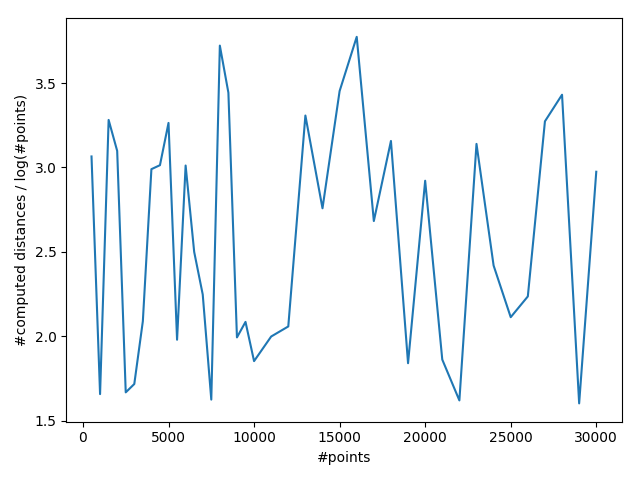
\includegraphics[width=0.7\textwidth]{pics/log_dependency_constant_ratio.png}
    \caption{Ratio $\log(\mbox{computed distances}) / n$ for ANN algorithm. Data is for uniformly distributed
    points.}
\end{figure}

\begin{figure}[ht]
    \label{fig:ann_dimension_dependency}
    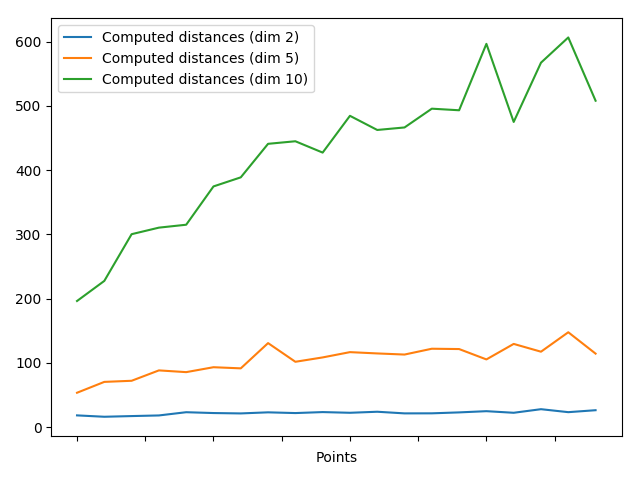
\includegraphics[width=0.7\textwidth]{pics/ann_computed_distances_dimension_dep.png}
    \caption{Number of computed distances for different dimensions. Points are chosen uniformly, $\eps = 0.01$.}
\end{figure}


We used the following methods of generating random points:
\begin{enumerate}
    \item Uniform. Points are sampled uniformly at random from the unit cube in $\R^d$.
    \item Normal. Points are sampled from the normal distribution.
\end{enumerate}
Query points were sampled from the uniform distribution on the cube $[-10, 10]^d$
and from the normal distribution centered at the origin with scale 100,
thus we get query points that are "inside" the point set and also "outside".
We sample data in dimensions up to 20 and for $\eps \in \Set{0.001, 0.005, 0.01, 0.05, 0.1}$,
the maximal number of points is $30,000$.

In order to empirically verify the upper bound $O(\log n)$,
we plot the number of computed distances divided
by the logarithm of the number of points in figure \ref{fig:ann_const_ratio} (for $d = 2$).
We see that this ratio, though fluctuating a lot, remains in the interval $[1,4]$. This not just confirms
the theoretical upper bound, but also shows that the algorithm in the low-dimensional case
really computes only a very small number of distances to the query point.
As expected, in high dimensions the algorithm does not perform as well.
In figure \ref{fig:ann_dimension_dependency} we plot the average number of computed distances
for $d = 2, 5, 10$. While for $d = 2$ the growth is hardly noticeable, for $d = 10$
the sublinearity of the growth becomes clear only when the number of points is relatively large,
approaching 30000.

% We also looked at the dependency on the density. Note that our algorithm is not invariant under scaling: if we multiply the metric
% by $\lambda$, we should also change $\eps$ to $\lambda \eps$, if we want
% the same behavior. Therefore we could \textit{a priori} expect some
% changes even if we change the parameters of the uniform distribution
% without changing epsilon. However,
% when we tested the algorithm on uniform data sampled from $[-a,a]^d$
% for $a \in \Set{1, 10, 100, 1000, 10000}$ and on normal data
% sampled from normal distribution with scales from the same set,
% we did not observe any significant difference.


%\section{Geometric concepts}

%We revise the concepts that were designed for nearest neighbor queries
%and metric approximation in metric spaces with low dimensionality.
%We will also review the computation methods and how they depend
%on the predicate ``$\dist(p_i,p_j)\leq t$?'' mentioned above.

%\paragraph{Notion of Dimensionality.}
%%
%Exansion constant, doubling dimension.

%\subsection{Cover trees}


%\subsection{WSPD}
%Given $s > 1$, two disjoint subsets $A, B$ of a metric space $(X, d)$ are called $s$-\textit{well-separated},
%if 
%\[
%\forall a \in A \, \forall b \in B \, d(a, b) \geq s \max(\diam(A), \diam(B))
%\]
%A well-separated pair decomposition (WSPD) is a set of unordered pairs of sets $\{ \{A_1, B_1 \}, 
%\dots, \{A_s, B_s\} \}$ such that each pair $\{A_i, B_i\}$ is $s$-well-separated, and for every unordered pair $\{a, b\}$ of distinct points of $X$ there exists a unique $j$ such that $a \in A_j$ and $b \in B_j$.
%The notion of WSPD was introduced by Callahan and Kosaraju \cite{cal-kos-wspd}.


%\subsection{Spanners}

%\subsection{Approximate Greedy Spannner}

%Suppose that we have fast algorithms for computing $\lambda$-approximation of $d(x,y)$.
%In other words, for every pair of points $x,y$ we can compute an interval $[c, \lambda c]$ that is guaranteed to contain 
%the true distance $d(x,y)$.  Note that for every interval of this form there exists 
%a unique $k \in \{1, \dots, N-1 \}$ such that $[c, \lambda c] \subset [\lambda^k, \lambda^{k+2}]$. 
%Indeed, $k = \lceil \log_{\lambda}(c) \rceil$.
%We also assume that we know the range of all possible values of $k$ and they are all non-negative,
%$k = 1\dots N$. We call the intervals $[\lambda^k, \lambda^{k+2}]$ \textit{buckets}, even though they are overlapping.
%Now we can formulate the algorithm for finding a spanner.

%\begin{algorithmic}
%\label{alg:local_init}
%\Function{Approximate greedy spanner}{$rho$}
%    \ForAll {pairs $x,y \in X$}
%    \State {Place $x, y$ into corresponding bucket }
%    \EndFor
%\EndFunction
%\end{algorithmic}

%We can use essentially the same proof as in \cite{bose2010computing}.
%Claim 1. If $s > \lambda^2 $ and $A, B$ are $s$-separated, then all pairs $(a, a')$, $(b, b')$ with $a, a' \in A$
%and $b, b' \in B$ are processed before any of the pairs $(a, b)$.

%Indeed, if $s > \lambda^2$, then for every points $a_1, a_2 \in A$ and $b \in B$
%we have $\lambda^2 d(a_1, a_2) < d(a_1, b)$. If $\dappr(a_1, a_2)$ and $\dappr(a_1, b)$ denote the $\lambda$-approximations
%of the corresponding distances, then the inequality $\frac{\dappr(a_1, b)}{\dappr(a_1, a_2)} > \lambda$
%holds , hence $(a_1, a_2)$ will be placed in the bucket that precedes the bucket of $(a_1, b)$.


%Claim 2. If $s > \max(\lambda^2, \frac{2t+2}{t-1})$ and $A, B$ are two $s$-well-separated subsets of $X$,
%then in the approximate greedy spanner computed by \ref{alg:approx_greedy_spanner} there is at most one edge between $A$ and $B$.

%Suppose that the pair $(a_1, b_1)$ with $a_1 \in A$, $b_1 \in B$ was processed and the edge $(a, b)$
%was added to the spanner. Then from claim 1 we know that we already have a $t$-spanner on $A$ and $B$.
%Consider another pair $(a_2, b_2)$. Let $G$ be the weighted graph we have immediately after the edge $(a_1, b_1)$ has been addedhttps://v2.overleaf.com/project/5bf6fa26032afa24d94383a5
%to the spanner. By claim 1
%$d_G(a_2, a_1) \leq td(a_2, a_1)$ and $d_G(b_1, b_2) \leq t d(b_1, b_2)$.
%By properties of WSPD, $d_G(a_1, b_1) = d(a_1, b_1) \leq (1 + \frac{2}{s})d(a_2, b_2)$
%and $t d(a_2, a_1) \leq \frac{t}{s} d(a_2, b_2)$, $t d(b_1, b_2) \leq \frac{t}{s} d(a_2, b_2)$.

%Combining these inequalities, we get

%\begin{equation}
%    \begin{split}
%        d_G(a_2, b_2) & \leq  d_G(a_2, a_1) + d_G(a_1, b_1) + d_G(b_1, b_2)  \\
%                      & \leq  \frac{t}{s} d(a_2, b_2) + (1 + \frac{2}{s})d(a_2, b_2) + \frac{t}{s} d(a_2, b_2) \\
%                      & =     (1 + \frac{2t + 2}{s}) d(a_2, b_2)
%    \end{split}
%\end{equation}

%Solving for $s$ the inequality $1 + \frac{2t + 2}{s} < t$ gives $s > \frac{2t+2}{t-1}$.


\section{Conclusion and Future Work}
\label{sec:conclusion}
We presented experimental evidence showing that in low
doubling dimension we can avoid many distance computations,
if we try to get as much information as possible from the triangle inequality
applied to the previously computed distance. The \textsc{BlindGreedy} spanner
performs especially well, being able to produce  sparse spanners even for small values of  $\eps$.
For the approximate nearest neighbor algorithm we proved a logarithmic upper bound,
and, even though the constant in the proof was very large, we demonstrated
experimentally that this does not show in practice.

The next step on the theoretical side could be proving some upper bound
for blind spanners; it is also interesting to look at other metric space
algorithms and data structures in the setting of expensive distance computation.
On the more applied side, the further development of this approach would
be to find finite spaces of low dimension in practically
important cases, like spaces of persistence diagrams or images endowed with Wasserstein (a.k.a. Earth Movers)
metric. We know that low-dimensional subspaces of functions do not necessarily produce
low-dimensional spaces of persistence diagrams, but there may be some conditions
which guarantee that dimension does not increase too much.
% An easy example: consider a fixed function $f$ to which we apply
% a finite-dimensional family of perturbations, $f(x) + g(x; \lambda_1, \dots, \lambda_n)$;
% for instance, each $\lambda_i$ is associated with some $x_i$ and adds a Gaussian noise
% scaled by $\lambda$.
% If the perturbations are very small, then they will produce some small wiggles on the function,
% and then the optimal matcih


\bibliography{bib}
\bibliographystyle{plain}


\end{document}
